%%%%%%%%%%%%%%%%%%%%%%%%%%%%%%%%%%%%%%%%%%%%%%%%%%%%%%%%%%%%%%%%%%%%%%
%%  Copyright by Wenliang Du.                                       %%
%%  This work is licensed under the Creative Commons                %%
%%  Attribution-NonCommercial-ShareAlike 4.0 International License. %%
%%  To view a copy of this license, visit                           %%
%%  http://creativecommons.org/licenses/by-nc-sa/4.0/.              %%
%%%%%%%%%%%%%%%%%%%%%%%%%%%%%%%%%%%%%%%%%%%%%%%%%%%%%%%%%%%%%%%%%%%%%%

\newcommand{\commonfolder}{../../common-files}

\documentclass[11pt]{article}

\usepackage[most]{tcolorbox}
\usepackage{times}
\usepackage{epsf}
\usepackage{epsfig}
\usepackage{amsmath, alltt, amssymb, xspace}
\usepackage{wrapfig}
\usepackage{fancyhdr}
\usepackage{url}
\usepackage{verbatim}
\usepackage{fancyvrb}
\usepackage{adjustbox}
\usepackage{listings}
\usepackage{color}
\usepackage{subfigure}
\usepackage{cite}
\usepackage{sidecap}
\usepackage{pifont}
\usepackage{mdframed}
\usepackage{textcomp}
\usepackage{enumitem}


% Horizontal alignment
\topmargin      -0.50in  % distance to headers
\oddsidemargin  0.0in
\evensidemargin 0.0in
\textwidth      6.5in
\textheight     8.9in 

\newcommand{\todo}[1]{
\vspace{0.1in}
\fbox{\parbox{6in}{TODO: #1}}
\vspace{0.1in}
}


\newcommand{\unix}{{\tt Unix}\xspace}
\newcommand{\linux}{{\tt Linux}\xspace}
\newcommand{\minix}{{\tt Minix}\xspace}
\newcommand{\ubuntu}{{\tt Ubuntu}\xspace}
\newcommand{\setuid}{{\tt Set-UID}\xspace}
\newcommand{\openssl} {\texttt{openssl}}


\pagestyle{fancy}
\lhead{\bfseries SEED Labs}
\chead{}
\rhead{\small \thepage}
\lfoot{}
\cfoot{}
\rfoot{}


\definecolor{dkgreen}{rgb}{0,0.6,0}
\definecolor{gray}{rgb}{0.5,0.5,0.5}
\definecolor{mauve}{rgb}{0.58,0,0.82}
\definecolor{lightgray}{gray}{0.90}


\lstset{%
  frame=none,
  language=,
  backgroundcolor=\color{lightgray},
  aboveskip=3mm,
  belowskip=3mm,
  showstringspaces=false,
%  columns=flexible,
  basicstyle={\small\ttfamily},
  numbers=none,
  numberstyle=\tiny\color{gray},
  keywordstyle=\color{blue},
  commentstyle=\color{dkgreen},
  stringstyle=\color{mauve},
  breaklines=true,
  breakatwhitespace=true,
  tabsize=3,
  columns=fullflexible,
  keepspaces=true,
  escapeinside={(*@}{@*)}
}

\newcommand{\newnote}[1]{
\vspace{0.1in}
\noindent
\fbox{\parbox{1.0\textwidth}{\textbf{Note:} #1}}
%\vspace{0.1in}
}


%% Submission
\newcommand{\seedsubmission}{You need to submit a detailed lab report, with screenshots,
to describe what you have done and what you have observed.
You also need to provide explanation
to the observations that are interesting or surprising.
Please also list the important code snippets followed by
explanation. Simply attaching code without any explanation will not
receive credits.}

%% Book
\newcommand{\seedbook}{\textit{Computer \& Internet Security: A Hands-on Approach}, 2nd
Edition, by Wenliang Du. See details at \url{https://www.handsonsecurity.net}.}

%% Videos
\newcommand{\seedisvideo}{\textit{Internet Security: A Hands-on Approach},
by Wenliang Du. See details at \url{https://www.handsonsecurity.net/video.html}.}

\newcommand{\seedcsvideo}{\textit{Computer Security: A Hands-on Approach},
by Wenliang Du. See details at \url{https://www.handsonsecurity.net/video.html}.}

%% Lab Environment
\newcommand{\seedenvironment}{This lab has been tested on our pre-built
Ubuntu 16.04 VM, which can be downloaded from the SEED website. }

\newcommand{\seedenvironmentA}{This lab has been tested on our pre-built
Ubuntu 16.04 VM, which can be downloaded from the SEED website. }

\newcommand{\seedenvironmentB}{This lab has been tested on our pre-built
Ubuntu 20.04 VM, which can be downloaded from the SEED website. }

\newcommand{\seedenvironmentAB}{This lab has been tested on our pre-built
Ubuntu 16.04 and 20.04 VMs, which can be downloaded from the SEED website. }

\newcommand{\nodependency}{Since we use containers to set up the lab environment, 
this lab does not depend too much on our SEED VM. You can do this lab
using other VMs or physical machines. }







\newcommand{\seedlabcopyright}[1]{
\vspace{0.1in}
\fbox{\parbox{6in}{\small Copyright \copyright\ {#1}\ \ by Wenliang Du.\\
      This work is licensed under a Creative Commons
      Attribution-NonCommercial-ShareAlike 4.0 International License.
      If you remix, transform, or build upon the material, 
      this copyright notice must be left intact, or reproduced in a way that is reasonable to
      the medium in which the work is being re-published.}}
\vspace{0.1in}
}






\newcommand{\heartFigs}{./Figs}

\lhead{\bfseries SEED Labs -- Heartbleed Attack}

\begin{document}

\begin{center}
{\LARGE Heartbleed Attack Lab}
\end{center}


\seedlabcopyright{2016}


% *******************************************
% SECTION
% ******************************************* 
\section{Overview}



The Heartbleed bug (CVE-2014-0160) is a severe implementation flaw in the
OpenSSL library, which enables attackers to steal data 
from the memory of the victim server. The contents of the stolen data
depend on what is there in the memory of the server. It could
potentially contain private keys, TLS session keys, user names,
passwords, credit cards, etc. The vulnerability is in the implementation of
the Heartbeat protocol,  which is used by SSL/TLS to keep the connection alive. 


The objective of this lab is for students to understand how serious this
vulnerability is, how the attack works, and how to fix the problem. The
affected OpenSSL version range is from {\tt 1.0.1} to {\tt 1.0.1f}. The
version in the SEEDUbuntu 12.04 VM is {\tt 1.0.1}. 



\paragraph{Readings and videos.}
Detailed coverage of the Heartbleed attack can be found in the following:

\begin{itemize}
\item Chapter 20 of the SEED Book, \seedbook
\item Section 11 of the SEED Lecture, \seedisvideo
\end{itemize}



\paragraph{Lab environment.} This lab has been tested on our pre-built
Ubuntu 12.04 VM, which can be downloaded from the SEED website.
If you are using our SEEDUbuntu 16.04 VM, this attack will not work, because the
vulnerability has already been patched.
You can download the SEEDUbuntu12.04 VM from the SEED web
site. If you have an Amazon EC2 account, you can find our VM from
the ``Community AMIs''. The name of the VM is
\texttt{SEEDUbuntu12.04-Generic}. It should be noted that
Amazon's site says that this is a 64-bit VM; that is incorrect. The VM is
32-bit. However, this incorrect information does not cause any problem.






% *******************************************
% SECTION
% ******************************************* 
\section{Lab Environment}

In this lab, we need to set up two VMs: one called attacker machine 
and the other called victim server.  We use the 
pre-built \texttt{SEEDUbuntu12.04} VM. The VMs need to use the 
\texttt{NAT-Network} adapter
for the network setting. This can be done by going to the VM settings,
picking Network, and clicking the Adaptor tag to switch the adapter to
\texttt{NAT-Network}. Make sure both VMs are on the same NAT-Network.

The website used in this attack can be any HTTPS website that uses SSL/TLS.
However, since it is illegal to attack a real website, we 
have set up a website in our VM, and conduct the attack on our own VM.
We use an open-source social network application called \texttt{ELGG},
and host it in the following URL: \url{https://www.heartbleedlabelgg.com}.

We need to modify the \texttt{/etc/hosts} file on the attacker
machine to map the server name to the IP address of 
the server VM. Search the following line in \texttt{/etc/hosts}, and 
replace the IP address \texttt{127.0.0.1} with the actual IP address of the
server VM that hosts the \texttt{ELGG} application.


\begin{lstlisting}
127.0.0.1	www.heartbleedlabelgg.com
\end{lstlisting}
 
 


% *******************************************
% SECTION
% ******************************************* 
\section{Lab Tasks}


Before working on the lab tasks, you need to understand how the heartbeat
protocol works.
The heartbeat protocol consists of two message types:
HeartbeatRequest packet and HeartbeatResponse packet. Client sends a
HeartbeatRequest packet to the server. When the server receives it, it 
sends back a copy of the received message in the HeartbeatResponse packet.
The goal is to keep the connection alive. 
%The protocol is illustrated in Figure~\ref{fig:big_picture}. 



% -------------------------------------------
% SUBSECTION
% ------------------------------------------- 
\subsection{Task 1: Launch the Heartbleed Attack}

In this task, students will launch the Heartbleed attack on 
our social network site and see what kind of damages can be achieved. 
The actual damage of the Heartbleed attack depends on what kind of
information is stored in the server memory. If there has not been much
activity on the server, you will not be able to steal useful data.
Therefore, we need to interact with the web server as legitimate users. Let us
do it as the administrator, and do the followings:
	  
  \begin{itemize} 
  \item Visit \texttt{https://www.heartbleedlabelgg.com} from your
        browser. 
  \item Login as the site administrator. (User Name:\texttt{admin}; Password:\texttt{seedelgg})
  \item Add Boby as friend. (Go to \texttt{More -> Members} and
	  click  \texttt{Boby -> Add Friend})
  \item Send Boby a private message.
  \end{itemize} 
	    

After you have done enough interaction as legitimate users, you can launch
the attack and see what information you can get out of the victim server. 
Writing the program to launch the Heartbleed attack from scratch is not
easy, because it requires the low-level knowledge of the Heartbeat
protocol. Fortunately, other people have already written the
attack code. Therefore, we will use the existing code to gain
first-hand experience in the Heartbleed attack.
The code that we use is called \texttt{attack.py},
which was originally written by Jared Stafford.
We made some small changes to the code for educational purposes.
You can download the code from the lab's web site, change its permission so
the file is executable. You can then run the attack code as follows:

\begin{lstlisting}
$ ./attack.py  www.heartbleedlabelgg.com
\end{lstlisting}
	   
You may need to run the attack code multiple times to get useful data. 
Try and see whether you can get the following information from the target
server. 

\begin{itemize} 
	\item User name and password.
	\item User's activity (what the user has done).
	\item The exact content of the private message.
\end{itemize} 
  
For each piece of secret that you steal from the Heartbleed attack, you need to
show the screen-dump as the proof and explain how you did the attack, 
and what your observations are.



% -------------------------------------------
% SUBSECTION
% ------------------------------------------- 
\subsection{Task 2: Find the Cause of the Heartbleed Vulnerability}

In this task, students will compare the outcome of the benign packet and
the malicious packet sent by the attacker code to find out the fundamental
cause of the Heartbleed vulnerability. 


The Heartbleed attack is based on the Heartbeat request. This request just
sends some data to the server, and the server will copy the data to its
response packet, so all
the data are echoed back.
In the normal case, suppose that the request includes 3 bytes of data "ABC",
so the length field has a value 3. The server will place the 
data in the memory, and copy 3 bytes from the beginning of the data to its
response packet. 
In the attack scenario, the request may contain 3 bytes of data, but 
the length field may say 1003. When the server constructs its response packet, it copies from the
starting of the data (i.e. ``ABC''), but it copies 1003 bytes, instead of 3 bytes. 
These extra 1000 types obviously do not come from the request packet; they come from the 
server's private memory, and they may contain other user's
information, secret keys, password, etc. 


\begin{figure}[htb]
\centering
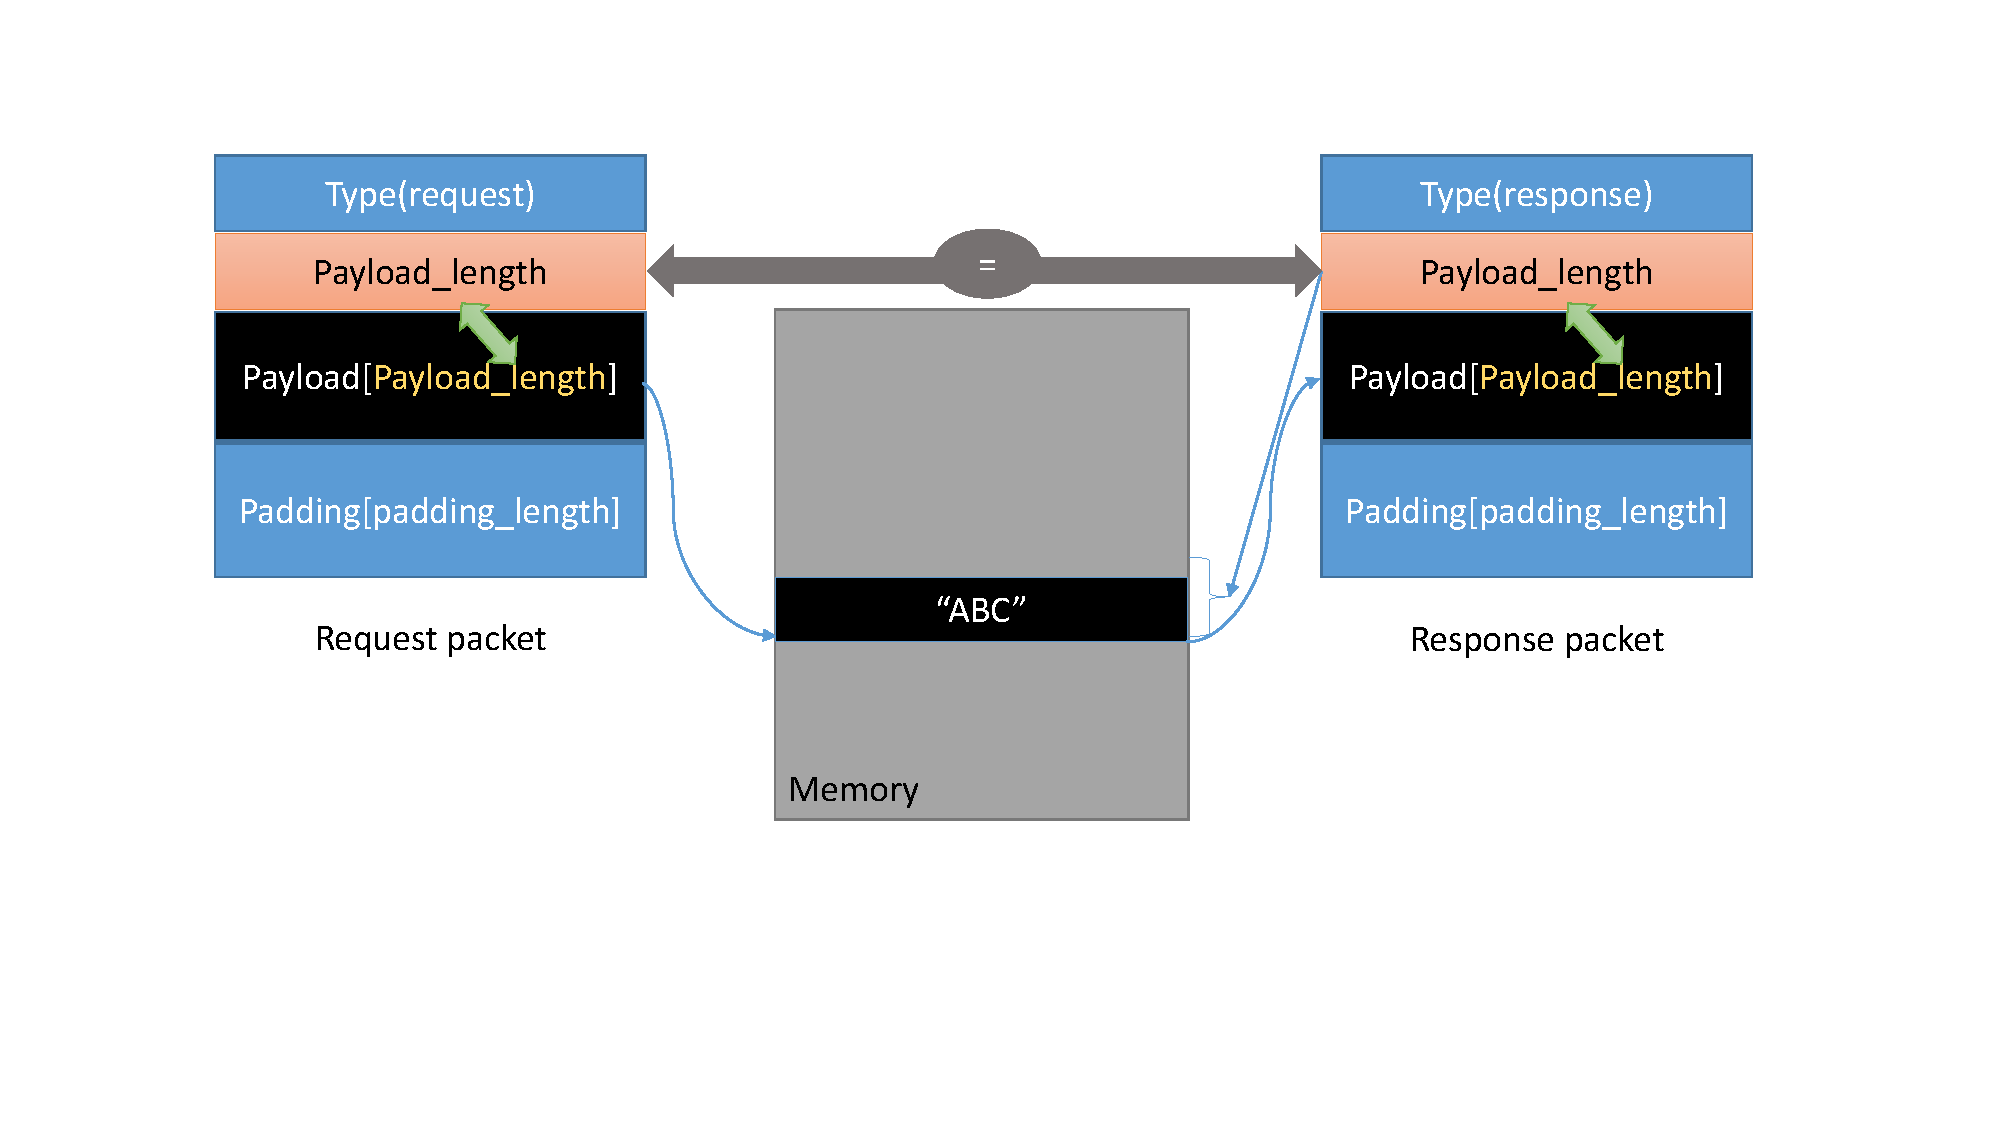
\includegraphics[width=0.8\textwidth]{\heartFigs/benign_packet.pdf}
\caption{The Benign Heartbeat Communication} 
\label{fig:benign_packet}
\end{figure}

In this task, we will play with the length field of the request.
First, let's understand how the Heartbeat response packet is built from 
Figure~\ref{fig:benign_packet}. When the Heartbeat request packet comes,
the server will parse the packet to get the payload and
the \texttt{Payload\_length} value (which is highlighted in 
Figure~\ref{fig:benign_packet}). Here, the payload is only a 3-byte string
\texttt{"ABC"} and the \texttt{Payload\_length} value is exactly 3. The server program will
blindly take this length value from the request packet. It then builds
the response packet by pointing to the memory storing \texttt{"ABC"} and copy 
\texttt{Payload\_length} bytes to the response payload. In
this way, the response packet would contain a 3-byte string \texttt{"ABC"}.

\begin{figure}[!htb]
\centering
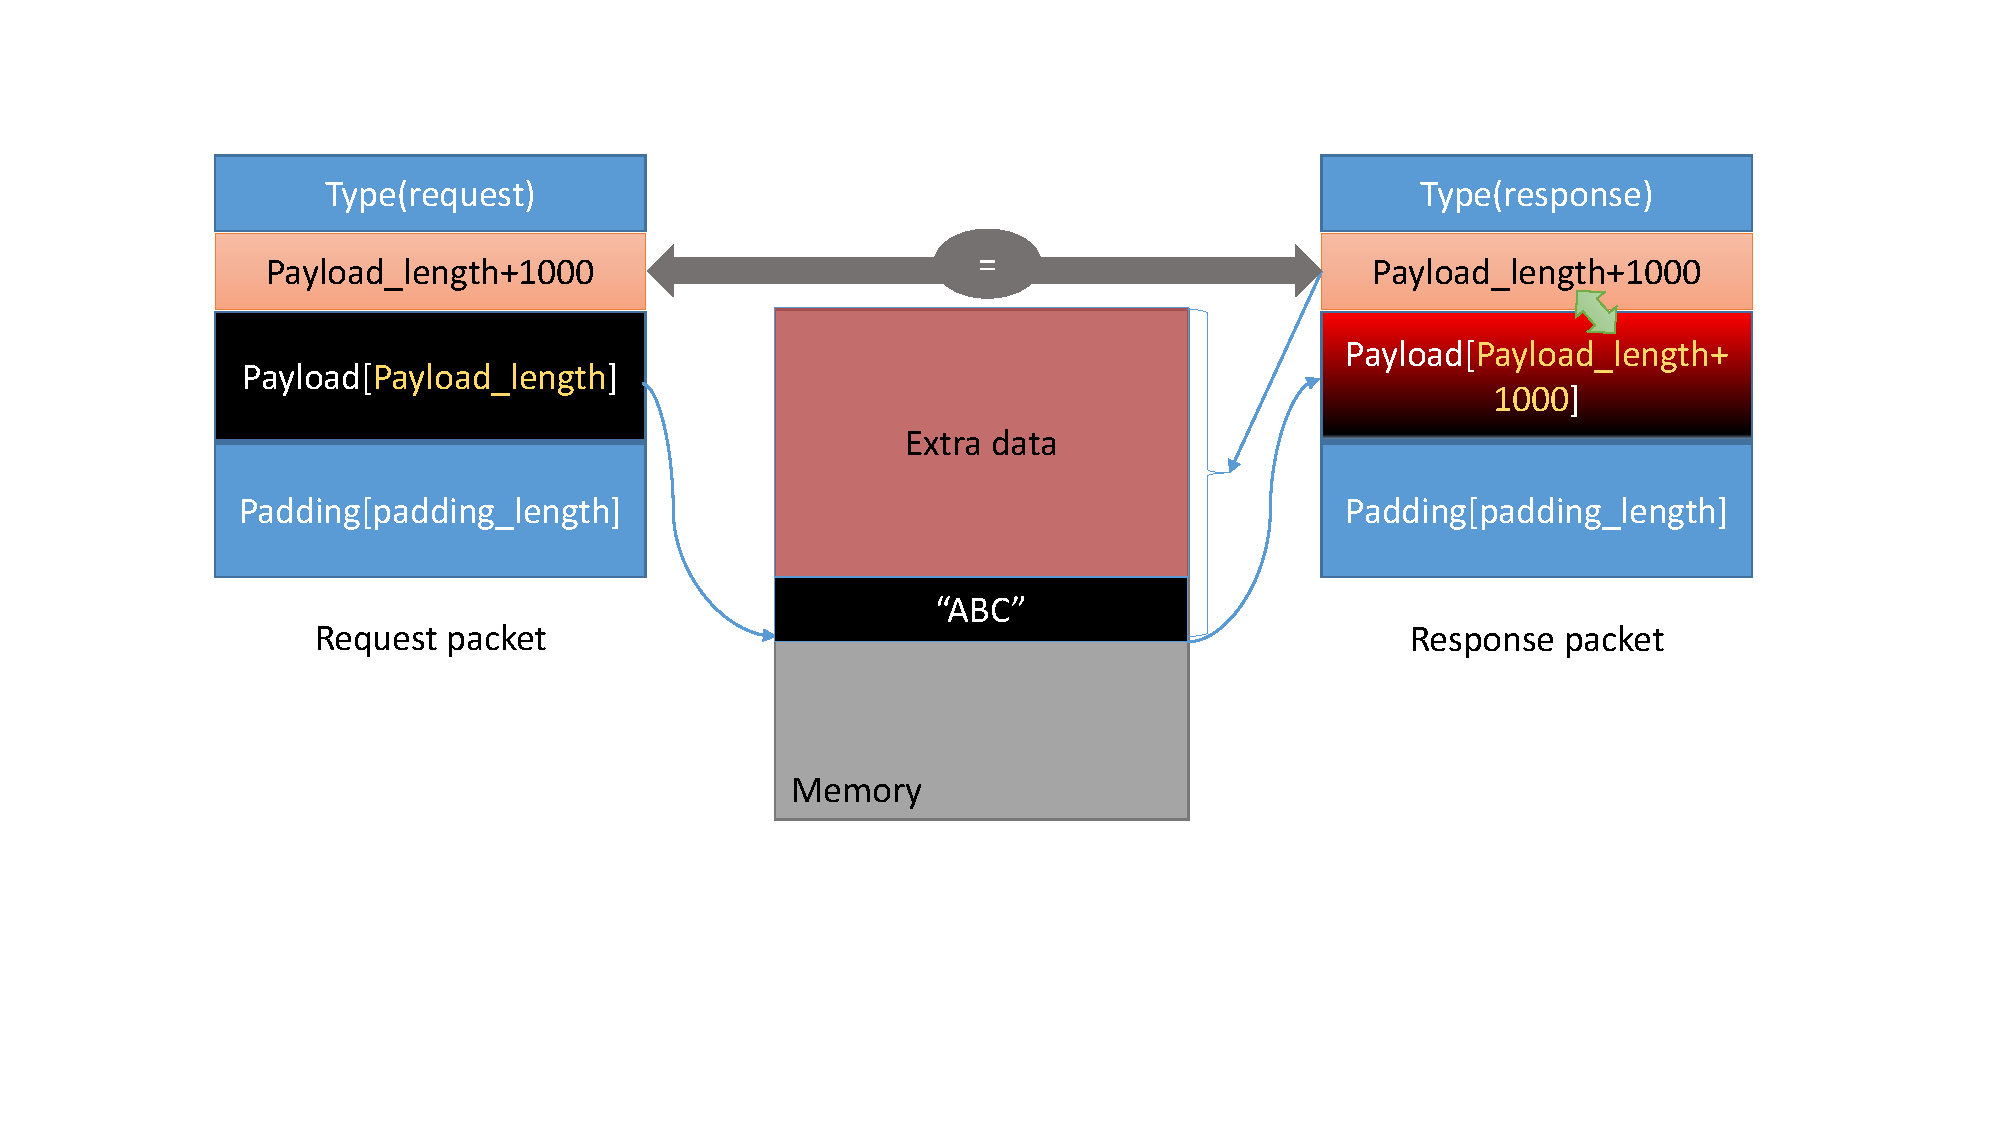
\includegraphics[width=0.8\textwidth]{\heartFigs/mal_packet.pdf}
\caption{The Heartbleed Attack Communication} 
\label{fig:mal_packet}
\end{figure}

We can launch the HeartBleed attack like what is shown in
Figure~\ref{fig:mal_packet}. We keep the same payload (3 bytes), but set
the \texttt{Payload\_length} field to 1003. The
server will again blindly take this \texttt{Payload\_length} value when building the response packet. This
time, the server program will point to the string \texttt{"ABC"} and copy 1003 bytes from the memory to
the response packet as a payload.  Besides the string "ABC", the extra 1000 bytes are copied
into the response packet, which could be anything from the memory, such as secret activity,
logging information, password and so on.



Our attack code allows
you to play with different \texttt{Payload\_length} values. By default, the
value is set to a quite large one (\texttt{0x4000}), but you can
reduce the size using the command option \texttt{"-l"} (letter ell)
or \texttt{"--length"} as shown in the following examples: 

\begin{lstlisting}
$./attack.py  www.heartbleedlabelgg.com  -l  0x015B 
$./attack.py  www.heartbleedlabelgg.com	 --length 83
\end{lstlisting}
 

Your task is to play with the attack program with different payload length
values and answer the
following questions:


\begin{itemize}
  \item {\bf Question 2.1:} As the length variable decreases, what kind of difference can you observe?

  \item {\bf Question 2.2:} As the length variable decreases, there is a boundary value for the input length
    variable.  At or below that boundary, the Heartbeat query will receive
    a response packet
    without attaching any extra data (which means the request is benign). Please find that
    boundary length.  You may need to try many
    different length values until the web server sends back the reply
    without extra data.  To help you with this, when the number of returned bytes is smaller
    than the expected length, the program will print \texttt{"Server processed malformed
    Heartbeat, but did not return any extra data."}
\end{itemize}




% -------------------------------------------
% SUBSECTION
% ------------------------------------------- 
\subsection{Task 3: Countermeasure and Bug Fix}

To fix the Heartbleed vulnerability, the best way is to update the OpenSSL
library to the newest version. This can be achieved using the following commands. 
It should be noted that once it is updated, it is hard to go back to the
vulnerable version. Therefore, make sure you have finished the previous
tasks before doing the update. You can also take a snapshot of your VM
before the update.


\begin{lstlisting}
$ sudo apt-get update
$ sudo apt-get upgrade
\end{lstlisting}


\paragraph{Task 3.1} Try your attack again after you have updated the
OpenSSL library. Please describe your observations. 



\paragraph{Task 3.2} The objective of this task is to figure out how to fix
the Heartbleed bug in the source code. The following C-style structure (not
exactly the same as the source code) is the format of the Heartbeat 
request/response packet. 


\begin{lstlisting}
struct {
   HeartbeatMessageType type; // 1 byte: request or the response
   uint16 payload_length;     // 2 byte: the length of the payload
   opaque payload[HeartbeatMessage.payload_length]; 
   opaque padding[padding_length]; 
} HeartbeatMessage;
\end{lstlisting}


The first field (1 byte) of the packet is the type information, 
and the second field (2 bytes) is the payload length, followed by the 
actual payload and paddings. The size of the payload should be the same as
the value in the \texttt{payload\_length} field, but in the attack
scenario, \texttt{payload\_length} can be set to a different value. The
following code snippet shows how the server 
copies the data from the request packet to the response packet. 



\begin{lstlisting}[caption={Process the Heartbeat request packet and generate the response packet}, 
      label=heartbleed:source]
/* Allocate memory for the response, size is 1 byte
 * message type, plus 2 bytes payload length, plus
 * payload, plus padding
 */

unsigned int payload;
unsigned int padding = 16; /* Use minimum padding */

// Read from type field first  
hbtype = *p++;   /* After this instruction, the pointer
                  * p will point to the payload_length field *.

// Read from the payload_length field 
// from the request packet 
n2s(p, payload); /* Function n2s(p, payload) reads 16 bits
                  * from pointer p and store the value 
                  * in the INT variable "payload". */
			  
			  
pl=p; // pl points to the beginning of the payload content
			  
if (hbtype == TLS1_HB_REQUEST)
{
     unsigned char *buffer, *bp;
     int r;

     /* Allocate memory for the response, size is 1 byte
      * message type, plus 2 bytes payload length, plus
      * payload, plus padding
      */

     buffer = OPENSSL_malloc(1 + 2 + payload + padding);
     bp = buffer;

     // Enter response type, length and copy payload 
     *bp++ = TLS1_HB_RESPONSE;
     s2n(payload, bp);
        
     // copy payload 
     memcpy(bp, pl, payload); /* pl is the pointer which 
                               * points to the beginning 
	                       * of the payload content */

     bp += payload;
			    
     // Random padding
     RAND_pseudo_bytes(bp, padding);			    

     // this function will copy the 3+payload+padding bytes
     // from the buffer and put them into the heartbeat response 
     // packet to send back to the request client side.
     r = ssl3_write_bytes(s, TLS1_RT_HEARTBEAT, buffer,
           3 + payload + padding); 
     OPENSSL_free(buffer);	   
}
\end{lstlisting}


Please point out the problem from the code in
Listing~\ref{heartbleed:source} and provide a solution to fix the
bug~(i.e., what modification is needed to fix the bug). You do not need to
recompile the code; just describe how you can fix the problem in your lab
report. 


Moreover, please comment on the following discussions by Alice, Bob, and
Eva regarding the fundamental cause of the Heartbleed vulnerability: 
Alice thinks the fundamental cause is missing the
boundary checking during the buffer copy; Bob thinks the cause is missing the
user input validation; Eva thinks that we can just delete the length value
from the packet to solve everything. 




% *******************************************
% SECTION
% ******************************************* 
\section{Submission}

%%%%%%%%%%%%%%%%%%%%%%%%%%%%%%%%%%%%%%%%

You need to submit a detailed lab report, with screenshots,
to describe what you have done and what you have observed.
You also need to provide explanation
to the observations that are interesting or surprising.
Please also list the important code snippets followed by
explanation. Simply attaching code without any explanation will not
receive credits.

%%%%%%%%%%%%%%%%%%%%%%%%%%%%%%%%%%%%%%%%



\end{document}
